\documentclass{standalone}

\usepackage{tikz}
\usepackage{standalone}
\usetikzlibrary{calc}
\usepackage{pgfplots}
\usepackage{color}

\begin{document}

    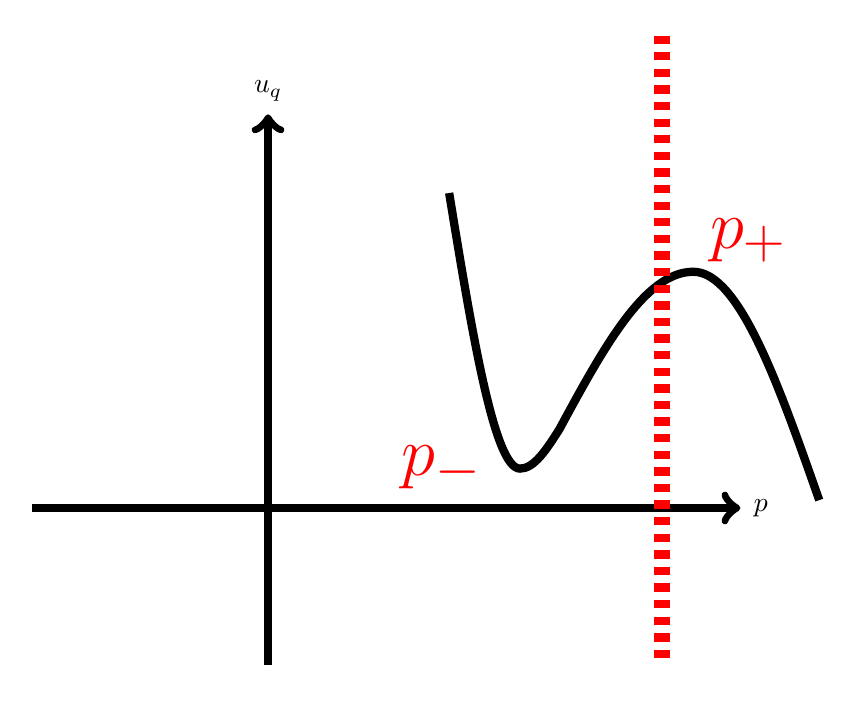
\begin{tikzpicture}

    \draw[->, line width=3pt] (-3, 0) -- (6, 0) node[right] {$p$};
    \draw[->, line width=3pt] (0,-2) -- (0,5) node[above] {$u_q$};

    \draw[line width=3pt] (2.3, 4) sin (3.2, 0.5) cos (3.7, 1) sin (5.4, 3) cos (7, 0.1);

    \node (0) at (2.2, 0.5) {\Huge{\textcolor{red}{\(p_{-}\)}}};
    \node (0) at (6.1, 3.4) {\Huge{\textcolor{red}{\(p_{+}\)}}};

	\draw [dashed, line width=2mm, red] (5,6) -- (5,-2);
    \end{tikzpicture}

\end{document}